\documentclass[10pt,a4paper,twocolumn,twoside]{article}
\usepackage[utf8]{inputenc}
\usepackage[catalan]{babel}
\usepackage{multicol}
\usepackage{graphicx}
\usepackage{fancyhdr}
\usepackage{times}
\usepackage{titlesec}
\usepackage{multirow}
\usepackage[top=2.5cm, bottom=1.3cm, left=1.2cm, right=1.2cm]{geometry}
\usepackage[figurename=Fig.,tablename=Taula,font={small,sf}]{caption}
\usepackage{subfig}
%\usepackage[font={small,sf}]{caption}

\usepackage{enumitem}
\setlist[itemize]{noitemsep}
\setlist[enumerate]{noitemsep}

\let\OLDthebibliography\thebibliography
\renewcommand\thebibliography[1]{
  \OLDthebibliography{#1}
  \setlength{\parskip}{0pt}
  \setlength{\itemsep}{0pt plus 0.3ex}
}

\pagestyle{fancy}
\fancyhf{}
\fancyhead[LO]{\textsf{\small $\mu$Projecte VC(GEI)-PSIV(GED), Escola d’Enginyeria (EE), Universitat Autònoma de Barcelona (UAB)}}
\fancyhead[RE]{\textsf{\small $\mu$Projecte VC(GEI)-PSIV(GED), Escola d’Enginyeria (EE), Universitat Autònoma de Barcelona (UAB)}}
\renewcommand{\headrulewidth}{0pt}

\titleformat*{\section}{\large\sffamily\scshape\bfseries}
\titleformat*{\subsection}{\normalsize\sffamily\bfseries}
\titleformat*{\subsubsection}{\normalsize\sffamily\slshape}

\begin{document}

{\sffamily
% Titol
\noindent\textbf{\LARGE Llegir i detectar tiquets de loteria}
% autors
\begin{center}
Marti Caixal i Joaniquet , Ricard López Olivares 
\end{center}

\bigskip
\bigskip

\noindent 
\textbf{Abstract}--- For this project of Visió per Computador del Grau d’Enginyeria Informàtica, it is quite a task to be able to know the numbers of a lottery ticket or similar through a photograph.

\bigskip

\noindent 
\textbf{Keywords}---Number detector, Homography, MSE, Lotery.
}
\bigskip

{\vrule depth 0pt height 0.5pt width 3cm\hspace{7.5pt}%
\raisebox{-3.5pt}{\fontfamily{pzd}\fontencoding{U}\fontseries{m}\fontshape{n}\fontsize{11}{12}\selectfont\char70}%
\hspace{7.5pt}\vrule depth 0pt height 0.5pt width 3cm\relax}

\bigskip


\section{Introducció}

Per aquest projecte de Visió per Computador del grau d’Enginyeria Informàtica es vol fer un treball per poder saber els números d’un tiquet de loteria o similar a través d’una fotografia.

\section{Objectius}

L’objectiu principal del projecte és, com ja s’ha comentat, poder obtenir els números d’un tiquet de loteria a través d’una imatge. Si més no, es pot separar en diferents subojectius independents els uns dels altres:

\begin{itemize}
	\item Transformar imatge: La fotografia de cada tiquet cal esperar que serà sempre agafada des d’un angle diferent. Així doncs, cada imatge tindrà una mida diferent, el tiquet estarà amb una orientació diferent, i en general no hi haurà correspondència entre les diferents imatges. L’objectiu d’aquest subapartat és aplicar una homografia per tal d’aconseguir una transofmació per cada imatge que ens permet tenir-les totes sobre un mateix pla. És a dir, que un cop s’hagi aplicat aquesta transformació, totes les imatges apareixen com si s’haguessin agafat des d’un mateix angle.\par
Per aconseguir fer aquesta homografia, caldrà tenir una imatge base i buscar uns punts de referència amb la resta d’imatges. La idea és fer-ho de forma automàtica i no pas manualment seleccionant els punts iguals d’ambdues imatges. D’aquesta manera s’aconsegueix que funcioni molt més ràpid per qualsevol imatge d’entrada que sigui d’un mateix tipus de tiquet de loteria
	\item Processar imatge: També s’ha de fer algunes correccions a les imatges. El més probable és que, quan es faci una binarització per passar-ho a blanc i negre i ens quedem només amb la informació de la imatge que ens interessa, hi hagi imperfections. Per tant, caldrà corregir-les mitjançant, segurament, operacions morfològiques. Tot i això, fins que no ens trobem amb el problema, no es pot saber exactament quin tipus de correccions es necessitarà.
	\item Separar números: Un cop es tenen els números identificats, la idea és separar-los en imatges independents per poder tractar amb ells individualment.
	\item Detectar números: El subobjectiu final és el més important, poder arribar a detectar quins números tenen els ticket de la loteria. Com que ara ja es té cada dígit del tiquet per separat, la idea per complir l’objectiu és veure la correlació que té cada un d’ell amb els 10 dígits que es tenen de base. El dígit que més correlació tingui serà el que dirà la predicció.
\end{itemize}

\section{Estat de l'art}

Actualment no hi ha cap sistema que haguem trobat que es dediqui a fer exactament el que vol fer el nostre projecte. \par
Sí que hi ha, però, moltes eines i treballs ja realitzats que compleixen algunes de les funcionalitats que necessitem nosaltres. \par
L’exemple que més hem trobat que ja està implementat i és quelcom similar, és la detecció dels números i lletres de les matrícules dels vehicles. A la pràctica és molt semblant a la detecció dels dígits a un bitllet de loteria. La majora d’aquest projectes fan la part de visió per computador i després fan servir xarxes neurals per aconseguir saber quin número és cada dígit. \cite{Sergio_Theodoridis}\par
També s’ha trobat que ja existeixen mètodes per trobar punts de referència entre dues fotografies. Mitjançant aquests punts és com es pot trobar la transformació necessària per DLT. \cite{Sandra_Kief}

\subsection{Dades: Exemples i fonts de dades}

Per realitzar aquest projecte es necessita un conjunt d’imatges de mostra. Per internet hi ha moltes fotografies que ja compleixen amb les nostres necessitats: vàries angles, varies qualitats i resolucions, etc… Addicionalment, un membre del grup té una àvia que guarda els números de loteria que ha jugat. Això ens permet aconseguir fotografies més exactes o específiques per fer les proves que faci falta. \par
A continuació es mostren dos fotografies d’exemple:

\begin{figure}[h]
 \centering
  \subfloat[fig1]{
   \label{f:fig2}
    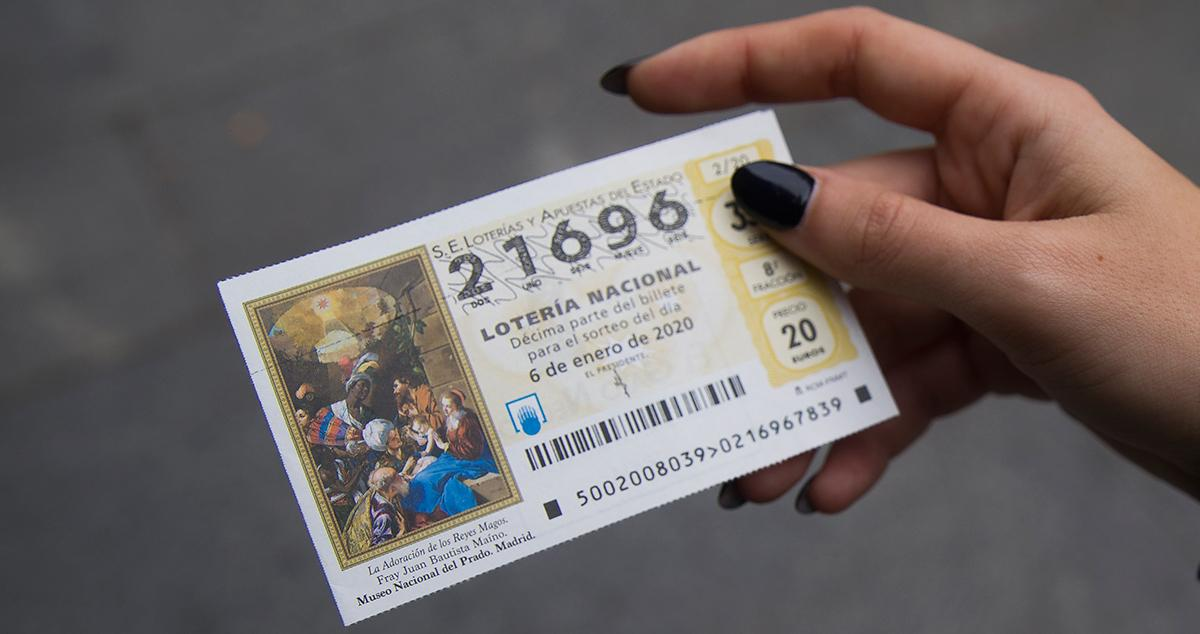
\includegraphics[width=0.235\textwidth]{figs/Fig2.jpeg}}
  \subfloat[fig2]{
   \label{f:fig1}
    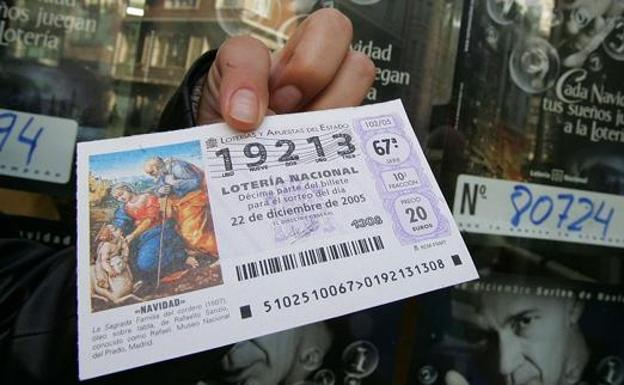
\includegraphics[width=0.2\textwidth]{figs/Fig1.jpg}}
  
 \label{f:Estat de lart}
\end{figure}


\section{Proposta}


 
\section{Experiments, resultats i anàlisi}



\subsection{Exemple de subsecció}





\section{Conclusions}




\begin{thebibliography}{9}
\bibitem{latex} \LaTeX. (21 d'Abril de 2021). A Wikibooks. http://en.wikibooks.org/wiki/LaTeX
\bibitem{Sergio_Theodoridis} Sergio Theodoridis, Konstantinos Koutroumbas, “Patther Recognitions” 3 edition.
\bibitem{Sandra_Kief} Sandra Kief, Danie Nuen, the Power of the Weisfeiler – Leman Algorithm to Decompose Graphs, SIAM Journal on Discrete Mathematics, 10.1137/20M1314987, 36, 1, (2022).


\end{thebibliography}
\end{document}

